\documentclass{standalone}

\usepackage{tikz}
\usetikzlibrary{angles,quotes}
\usepackage{amsmath,amssymb,amsfonts}

\usepackage{pgfplots}
\definecolor{darkgreen}{rgb}{0.0, 0.42, 0.24}
\definecolor{amethyst}{rgb}{0.6, 0.4, 0.8}

\pgfplotsset{compat=newest}
\pgfplotsset{every axis/.append style={
                     tick label style={font=\footnotesize},
                 }}


\begin{document}
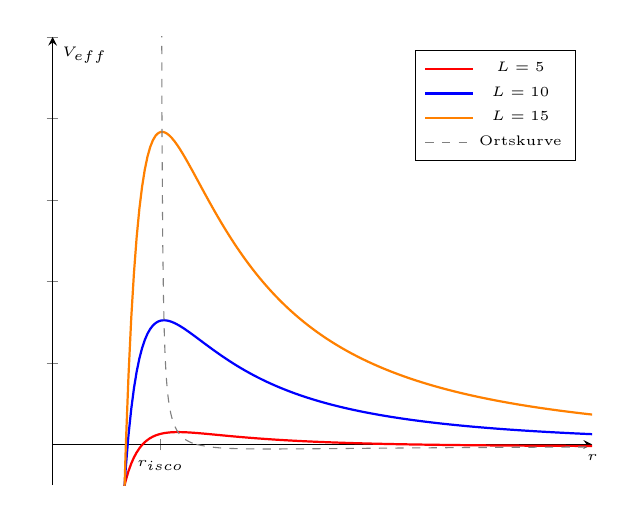
\begin{tikzpicture}
        \begin{axis}[xmin=0,xmax=15,ymin=-0.5,ymax=5,
        axis lines = middle,
        xlabel=$r$,
        ylabel=$V_{eff}$,
        label style={font=\tiny},
        tick label style={font=\tiny},
        xtick={3},
        xticklabels={$r_{isco}$},
        xticklabel style={anchor=north},
        xlabel style={anchor=north},
        yticklabels=false,
        domain=0:15,
        restrict y to domain=-5:10,
        legend pos =north east,
        legend style={font=\tiny}]
            \addplot[color=red,samples=200,thick]{-1/x+25/(2*x^2)-25/x^3};
           \addplot[color=blue,samples=200,thick]{-1/x+100/(2*x^2)-100/x^3};
           \addplot[color=orange,samples=200,thick]{-1/x+15^2/(2*x^2)-15^2/x^3};
           \addplot[color=gray,dashed,samples=50,domain=3:4]{1/(6*(x-3))-2/(3*x)};
           \addplot[color=gray,dashed,samples=50,domain=4:20]{1/(6*(x-3))-2/(3*x)};
           \addlegendentry{$L=5$}
           \addlegendentry{$L=10$}
           \addlegendentry{$L=15$}
           \addlegendentry{Ortskurve}
        \end{axis}
    \end{tikzpicture}
\end{document}